% Options for packages loaded elsewhere
\PassOptionsToPackage{unicode}{hyperref}
\PassOptionsToPackage{hyphens}{url}
\documentclass[
]{article}
\usepackage{xcolor}
\usepackage[margin=1in]{geometry}
\usepackage{amsmath,amssymb}
\setcounter{secnumdepth}{5}
\usepackage{iftex}
\ifPDFTeX
  \usepackage[T1]{fontenc}
  \usepackage[utf8]{inputenc}
  \usepackage{textcomp} % provide euro and other symbols
\else % if luatex or xetex
  \usepackage{unicode-math} % this also loads fontspec
  \defaultfontfeatures{Scale=MatchLowercase}
  \defaultfontfeatures[\rmfamily]{Ligatures=TeX,Scale=1}
\fi
\usepackage{lmodern}
\ifPDFTeX\else
  % xetex/luatex font selection
\fi
% Use upquote if available, for straight quotes in verbatim environments
\IfFileExists{upquote.sty}{\usepackage{upquote}}{}
\IfFileExists{microtype.sty}{% use microtype if available
  \usepackage[]{microtype}
  \UseMicrotypeSet[protrusion]{basicmath} % disable protrusion for tt fonts
}{}
\makeatletter
\@ifundefined{KOMAClassName}{% if non-KOMA class
  \IfFileExists{parskip.sty}{%
    \usepackage{parskip}
  }{% else
    \setlength{\parindent}{0pt}
    \setlength{\parskip}{6pt plus 2pt minus 1pt}}
}{% if KOMA class
  \KOMAoptions{parskip=half}}
\makeatother
\usepackage{color}
\usepackage{fancyvrb}
\newcommand{\VerbBar}{|}
\newcommand{\VERB}{\Verb[commandchars=\\\{\}]}
\DefineVerbatimEnvironment{Highlighting}{Verbatim}{commandchars=\\\{\}}
% Add ',fontsize=\small' for more characters per line
\usepackage{framed}
\definecolor{shadecolor}{RGB}{248,248,248}
\newenvironment{Shaded}{\begin{snugshade}}{\end{snugshade}}
\newcommand{\AlertTok}[1]{\textcolor[rgb]{0.94,0.16,0.16}{#1}}
\newcommand{\AnnotationTok}[1]{\textcolor[rgb]{0.56,0.35,0.01}{\textbf{\textit{#1}}}}
\newcommand{\AttributeTok}[1]{\textcolor[rgb]{0.13,0.29,0.53}{#1}}
\newcommand{\BaseNTok}[1]{\textcolor[rgb]{0.00,0.00,0.81}{#1}}
\newcommand{\BuiltInTok}[1]{#1}
\newcommand{\CharTok}[1]{\textcolor[rgb]{0.31,0.60,0.02}{#1}}
\newcommand{\CommentTok}[1]{\textcolor[rgb]{0.56,0.35,0.01}{\textit{#1}}}
\newcommand{\CommentVarTok}[1]{\textcolor[rgb]{0.56,0.35,0.01}{\textbf{\textit{#1}}}}
\newcommand{\ConstantTok}[1]{\textcolor[rgb]{0.56,0.35,0.01}{#1}}
\newcommand{\ControlFlowTok}[1]{\textcolor[rgb]{0.13,0.29,0.53}{\textbf{#1}}}
\newcommand{\DataTypeTok}[1]{\textcolor[rgb]{0.13,0.29,0.53}{#1}}
\newcommand{\DecValTok}[1]{\textcolor[rgb]{0.00,0.00,0.81}{#1}}
\newcommand{\DocumentationTok}[1]{\textcolor[rgb]{0.56,0.35,0.01}{\textbf{\textit{#1}}}}
\newcommand{\ErrorTok}[1]{\textcolor[rgb]{0.64,0.00,0.00}{\textbf{#1}}}
\newcommand{\ExtensionTok}[1]{#1}
\newcommand{\FloatTok}[1]{\textcolor[rgb]{0.00,0.00,0.81}{#1}}
\newcommand{\FunctionTok}[1]{\textcolor[rgb]{0.13,0.29,0.53}{\textbf{#1}}}
\newcommand{\ImportTok}[1]{#1}
\newcommand{\InformationTok}[1]{\textcolor[rgb]{0.56,0.35,0.01}{\textbf{\textit{#1}}}}
\newcommand{\KeywordTok}[1]{\textcolor[rgb]{0.13,0.29,0.53}{\textbf{#1}}}
\newcommand{\NormalTok}[1]{#1}
\newcommand{\OperatorTok}[1]{\textcolor[rgb]{0.81,0.36,0.00}{\textbf{#1}}}
\newcommand{\OtherTok}[1]{\textcolor[rgb]{0.56,0.35,0.01}{#1}}
\newcommand{\PreprocessorTok}[1]{\textcolor[rgb]{0.56,0.35,0.01}{\textit{#1}}}
\newcommand{\RegionMarkerTok}[1]{#1}
\newcommand{\SpecialCharTok}[1]{\textcolor[rgb]{0.81,0.36,0.00}{\textbf{#1}}}
\newcommand{\SpecialStringTok}[1]{\textcolor[rgb]{0.31,0.60,0.02}{#1}}
\newcommand{\StringTok}[1]{\textcolor[rgb]{0.31,0.60,0.02}{#1}}
\newcommand{\VariableTok}[1]{\textcolor[rgb]{0.00,0.00,0.00}{#1}}
\newcommand{\VerbatimStringTok}[1]{\textcolor[rgb]{0.31,0.60,0.02}{#1}}
\newcommand{\WarningTok}[1]{\textcolor[rgb]{0.56,0.35,0.01}{\textbf{\textit{#1}}}}
\usepackage{graphicx}
\makeatletter
\newsavebox\pandoc@box
\newcommand*\pandocbounded[1]{% scales image to fit in text height/width
  \sbox\pandoc@box{#1}%
  \Gscale@div\@tempa{\textheight}{\dimexpr\ht\pandoc@box+\dp\pandoc@box\relax}%
  \Gscale@div\@tempb{\linewidth}{\wd\pandoc@box}%
  \ifdim\@tempb\p@<\@tempa\p@\let\@tempa\@tempb\fi% select the smaller of both
  \ifdim\@tempa\p@<\p@\scalebox{\@tempa}{\usebox\pandoc@box}%
  \else\usebox{\pandoc@box}%
  \fi%
}
% Set default figure placement to htbp
\def\fps@figure{htbp}
\makeatother
\setlength{\emergencystretch}{3em} % prevent overfull lines
\providecommand{\tightlist}{%
  \setlength{\itemsep}{0pt}\setlength{\parskip}{0pt}}
\usepackage[]{natbib}
\bibliographystyle{plainnat}
\usepackage{bookmark}
\IfFileExists{xurl.sty}{\usepackage{xurl}}{} % add URL line breaks if available
\urlstyle{same}
\hypersetup{
  pdftitle={Lab 02 - Global plastic waste},
  pdfauthor={Tina Huynh},
  hidelinks,
  pdfcreator={LaTeX via pandoc}}

\title{Lab 02 - Global plastic waste}
\author{Tina Huynh}
\date{}

\begin{document}
\maketitle

{
\setcounter{tocdepth}{2}
\tableofcontents
}
Plastic pollution is a major and growing problem, negatively affecting
oceans and wildlife health.
\href{https://ourworldindata.org/plastic-pollution}{Our World in Data}
has a lot of great data at various levels including globally, per
country, and over time. For this lab we focus on data from 2010.

Additionally, National Geographic ran a data visualization communication
contest on plastic waste as seen
\href{https://www.nationalgeographic.org/funding-opportunities/innovation-challenges/plastic/dataviz/}{here}.

\section{Learning goals}\label{learning-goals}

\begin{itemize}
\tightlist
\item
  Visualising numerical and categorical data and interpreting
  visualisations
\item
  Recreating visualizations
\item
  Getting more practice using with R, RStudio, Git, and GitHub
\end{itemize}

\section{Getting started}\label{getting-started}

Go to the course GitHub organization and locate your assignment repo,
which should be named
\texttt{lab-02-plastic-waste-YOUR\_GITHUB\_USERNAME}. If you're in the
right place, it should look like the following.

\pandocbounded{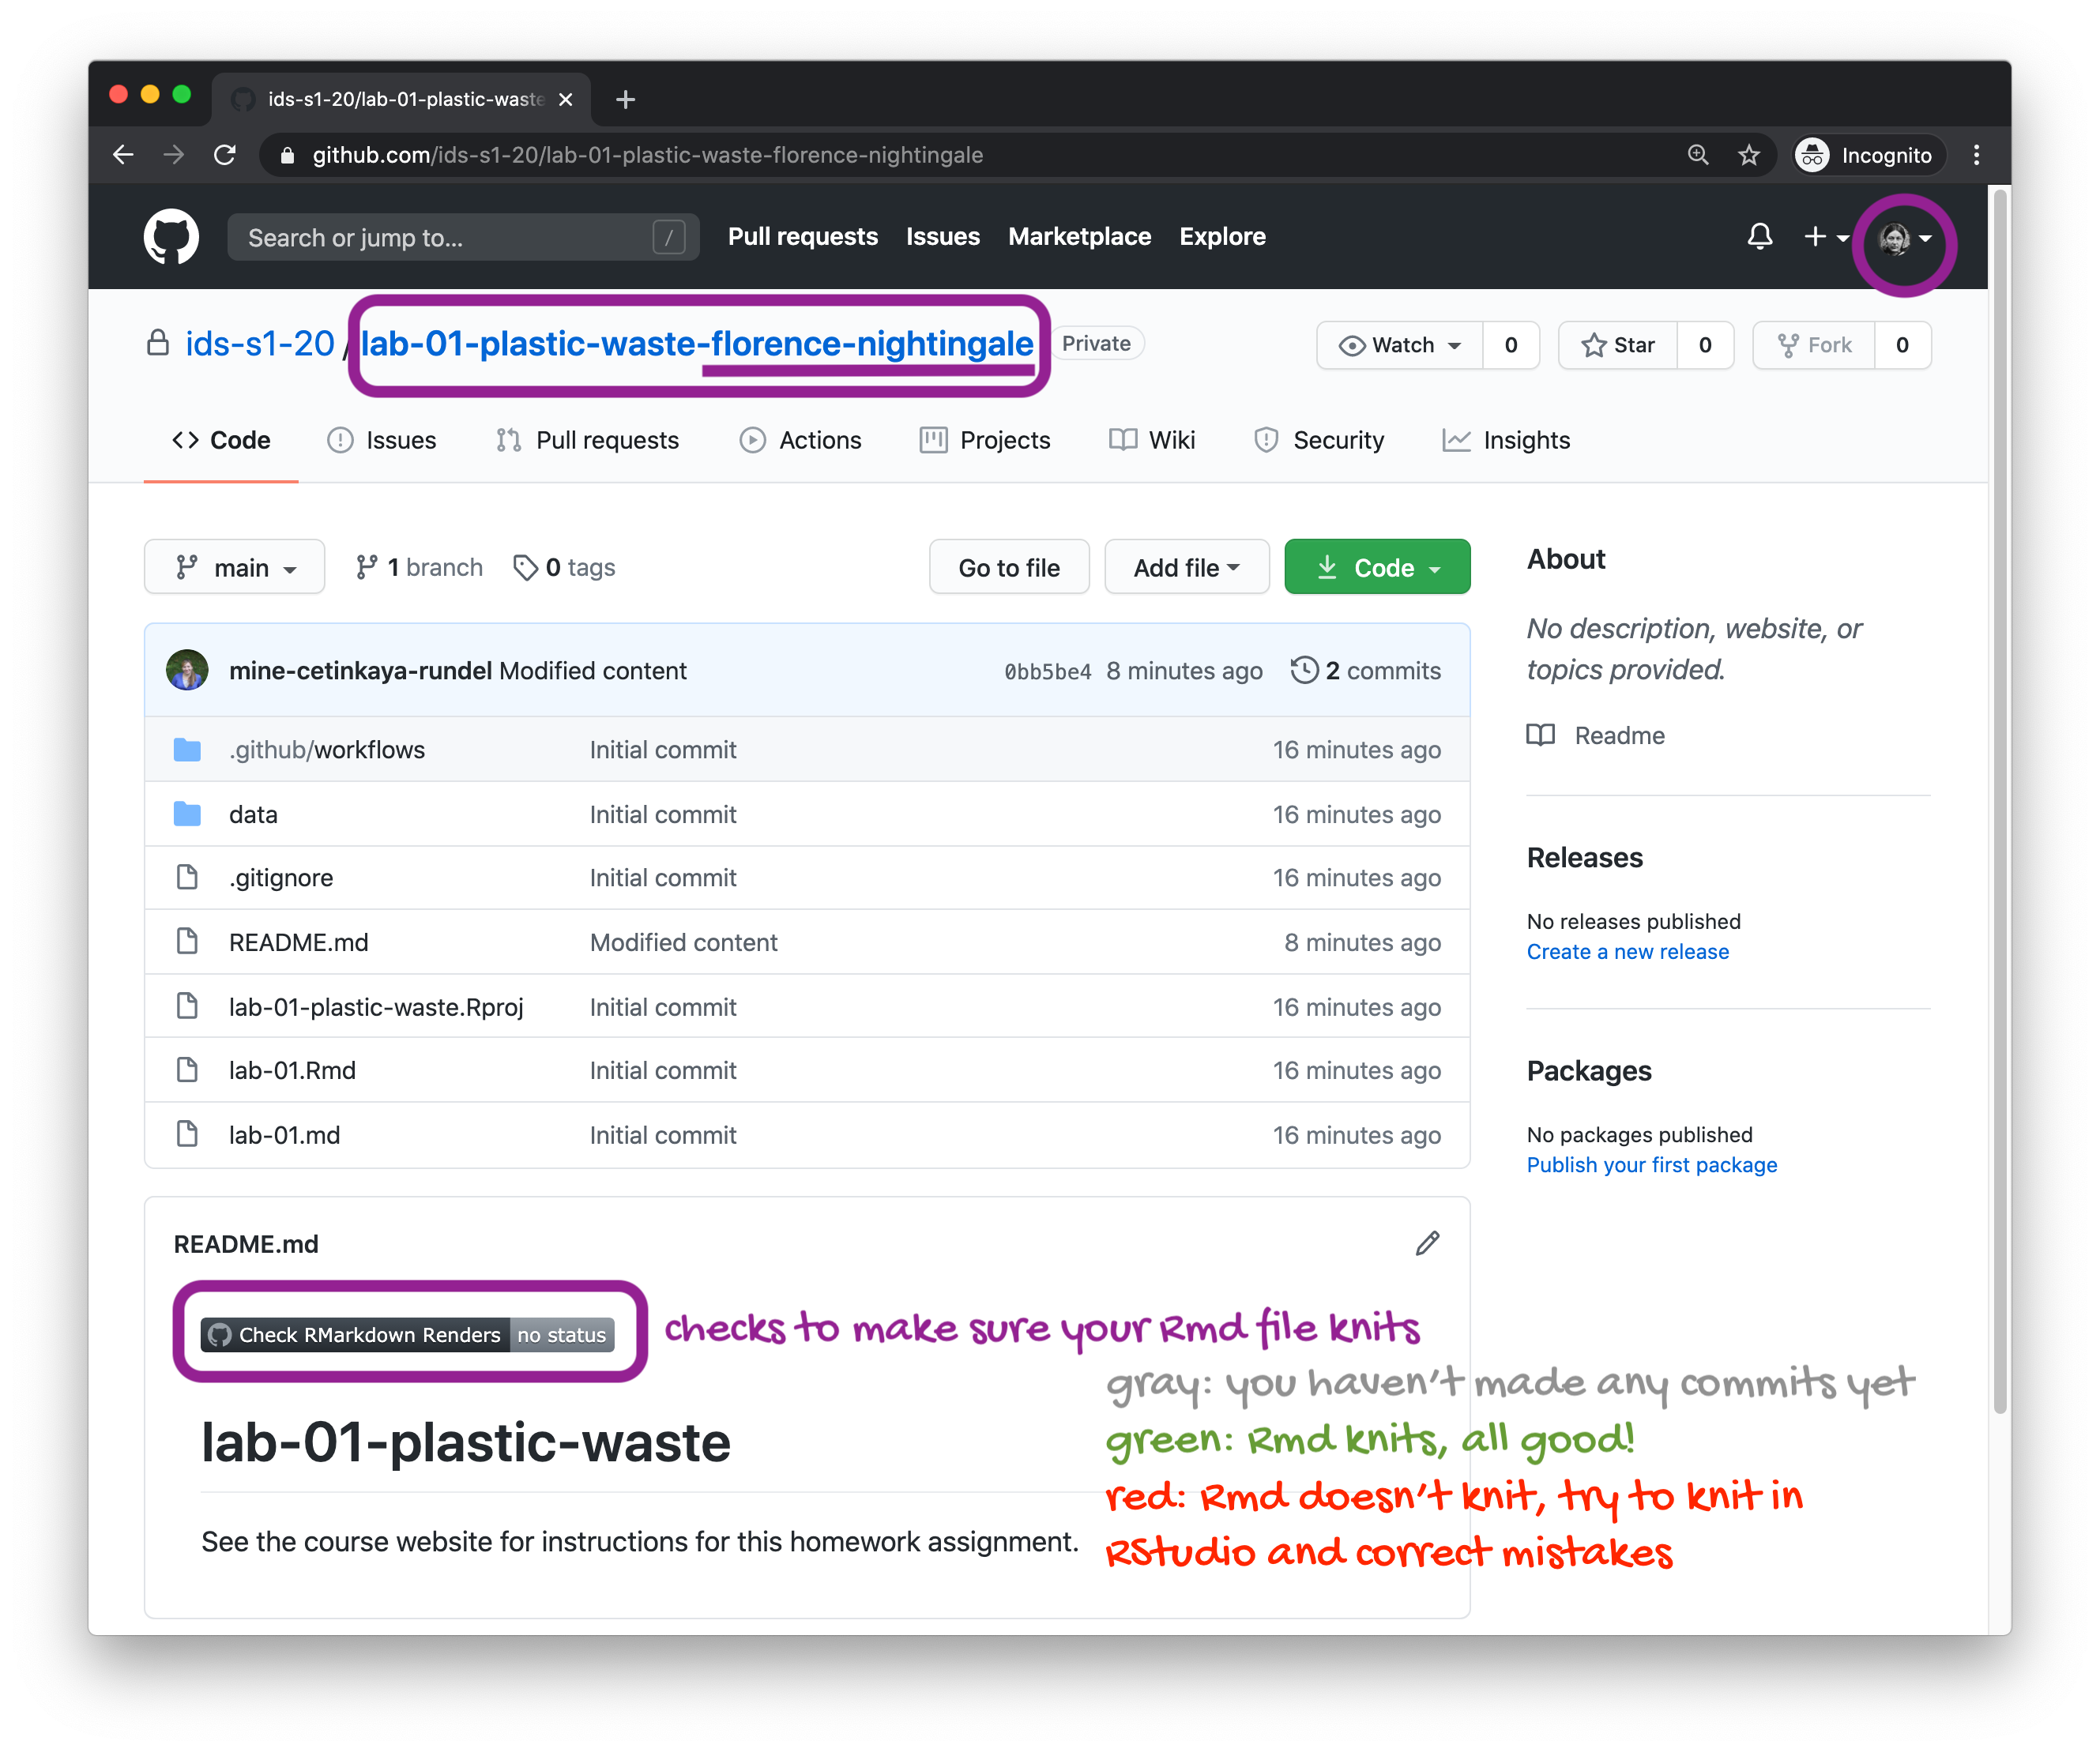
\includegraphics[keepaspectratio]{img/repo-begin.png}}

Grab the URL of the repo, and clone it in RStudio. Refer to
\href{https://ids-s1-20.github.io/homework/hw-00/hw-00-pet-names.html}{HW
00} if you would like to see step-by-step instructions for cloning a
repo into an RStudio project.

First, open the R Markdown document \texttt{lab-02.Rmd} and Knit it.
Make sure it compiles without errors. The output will be in the file
markdown \texttt{.md} file with the same name.

\section{Packages}\label{packages}

We'll use the \textbf{tidyverse} package for this analysis. Run the
following code in the Console to load this package.

\begin{Shaded}
\begin{Highlighting}[]
\FunctionTok{library}\NormalTok{(tidyverse)}
\end{Highlighting}
\end{Shaded}

\begin{verbatim}
## -- Attaching core tidyverse packages ------------------------ tidyverse 2.0.0 --
## v dplyr     1.1.4     v readr     2.1.5
## v forcats   1.0.0     v stringr   1.5.1
## v ggplot2   3.5.2     v tibble    3.3.0
## v lubridate 1.9.4     v tidyr     1.3.1
## v purrr     1.1.0     
## -- Conflicts ------------------------------------------ tidyverse_conflicts() --
## x dplyr::filter() masks stats::filter()
## x dplyr::lag()    masks stats::lag()
## i Use the conflicted package (<http://conflicted.r-lib.org/>) to force all conflicts to become errors
\end{verbatim}

\begin{Shaded}
\begin{Highlighting}[]
\FunctionTok{library}\NormalTok{(scales) }\CommentTok{\# nice axis labels}
\end{Highlighting}
\end{Shaded}

\begin{verbatim}
## 
## Attaching package: 'scales'
## 
## The following object is masked from 'package:purrr':
## 
##     discard
## 
## The following object is masked from 'package:readr':
## 
##     col_factor
\end{verbatim}

\begin{Shaded}
\begin{Highlighting}[]
\FunctionTok{library}\NormalTok{(janitor) }\CommentTok{\# tabulations \& clean names}
\end{Highlighting}
\end{Shaded}

\begin{verbatim}
## 
## Attaching package: 'janitor'
## 
## The following objects are masked from 'package:stats':
## 
##     chisq.test, fisher.test
\end{verbatim}

\section{Data}\label{data}

The dataset for this assignment can be found as a csv file in the
\texttt{data} folder of your repository. You can read it in using the
following.

\begin{Shaded}
\begin{Highlighting}[]
\NormalTok{plastic\_waste }\OtherTok{\textless{}{-}} \FunctionTok{read\_csv}\NormalTok{(}\StringTok{"data/plastic{-}waste.csv"}\NormalTok{) }\SpecialCharTok{\%\textgreater{}\%}
  \FunctionTok{clean\_names}\NormalTok{()}
\end{Highlighting}
\end{Shaded}

\begin{verbatim}
## Rows: 240 Columns: 10
## -- Column specification --------------------------------------------------------
## Delimiter: ","
## chr (3): code, entity, continent
## dbl (7): year, gdp_per_cap, plastic_waste_per_cap, mismanaged_plastic_waste_...
## 
## i Use `spec()` to retrieve the full column specification for this data.
## i Specify the column types or set `show_col_types = FALSE` to quiet this message.
\end{verbatim}

The variable descriptions are as follows:

\begin{itemize}
\tightlist
\item
  \texttt{code}: 3 Letter country code
\item
  \texttt{entity}: Country name
\item
  \texttt{continent}: Continent name
\item
  \texttt{year}: Year
\item
  \texttt{gdp\_per\_cap}: GDP per capita constant 2011 international \$,
  rate
\item
  \texttt{plastic\_waste\_per\_cap}: Amount of plastic waste per capita
  in kg/day
\item
  \texttt{mismanaged\_plastic\_waste\_per\_cap}: Amount of mismanaged
  plastic waste per capita in kg/day
\item
  \texttt{mismanaged\_plastic\_waste}: Tonnes of mismanaged plastic
  waste
\item
  \texttt{coastal\_pop}: Number of individuals living on/near coast
\item
  \texttt{total\_pop}: Total population according to Gapminder
\end{itemize}

\section{Warm up}\label{warm-up}

\begin{itemize}
\tightlist
\item
  Recall that RStudio is divided into four panes. Without looking, can
  you name them all and briefly describe their purpose?
\item
  Verify that the dataset has loaded into the Environment. How many
  observations are in the dataset? Clicking on the dataset in the
  Environment will allow you to inspect it more carefully.
  Alternatively, you can type \texttt{View(plastic\_waste)} into the
  Console to do this.
\end{itemize}

\begin{Shaded}
\begin{Highlighting}[]
\NormalTok{**Hint:** If you\textquotesingle{}re not sure, run the command \textasciigrave{}?NA\textasciigrave{} which will lead you to the documentation.}
\end{Highlighting}
\end{Shaded}

\begin{Shaded}
\begin{Highlighting}[]
\FunctionTok{glimpse}\NormalTok{(plastic\_waste)}
\end{Highlighting}
\end{Shaded}

\begin{verbatim}
## Rows: 240
## Columns: 10
## $ code                             <chr> "AFG", "ALB", "DZA", "ASM", "AND", "A~
## $ entity                           <chr> "Afghanistan", "Albania", "Algeria", ~
## $ continent                        <chr> "Asia", "Europe", "Africa", "Oceania"~
## $ year                             <dbl> 2010, 2010, 2010, 2010, 2010, 2010, 2~
## $ gdp_per_cap                      <dbl> 1614.255, 9927.182, 12870.603, NA, NA~
## $ plastic_waste_per_cap            <dbl> NA, 0.069, 0.144, NA, NA, 0.062, 0.25~
## $ mismanaged_plastic_waste_per_cap <dbl> NA, 0.032, 0.086, NA, NA, 0.045, 0.01~
## $ mismanaged_plastic_waste         <dbl> NA, 29705, 520555, NA, NA, 62528, 52,~
## $ coastal_pop                      <dbl> NA, 2530533, 16556580, NA, NA, 379004~
## $ total_pop                        <dbl> 31411743, 3204284, 35468208, 68420, 8~
\end{verbatim}

\begin{Shaded}
\begin{Highlighting}[]
\FunctionTok{nrow}\NormalTok{(plastic\_waste)}
\end{Highlighting}
\end{Shaded}

\begin{verbatim}
## [1] 240
\end{verbatim}

Interpretation: \texttt{glimpse()} confirms expected columns and types;
\texttt{nrow()} reports the number of rows (observations) present in
your local CSV.

\begin{itemize}
\tightlist
\item
  Have a quick look at the data and notice that there are cells taking
  the value \texttt{NA} -- what does this mean?
\end{itemize}

\textbf{Q: What does \texttt{NA} mean?}

\textbf{A:} \texttt{NA} represents a \textbf{missing value} (unknown/not
recorded). Many functions propagate \texttt{NA} unless you set
\texttt{na.rm\ =\ TRUE} or handle missingness explicitly (e.g.,
imputation, filtering).

\section{Exercises}\label{exercises}

Let's start by taking a look at the distribution of plastic waste per
capita in 2010.

\begin{Shaded}
\begin{Highlighting}[]
\FunctionTok{ggplot}\NormalTok{(}\AttributeTok{data =}\NormalTok{ plastic\_waste, }\FunctionTok{aes}\NormalTok{(}\AttributeTok{x =}\NormalTok{ plastic\_waste\_per\_cap)) }\SpecialCharTok{+}
  \FunctionTok{geom\_histogram}\NormalTok{(}\AttributeTok{binwidth =} \FloatTok{0.2}\NormalTok{)}
\end{Highlighting}
\end{Shaded}

\begin{verbatim}
## Warning: Removed 51 rows containing non-finite outside the scale range
## (`stat_bin()`).
\end{verbatim}

\pandocbounded{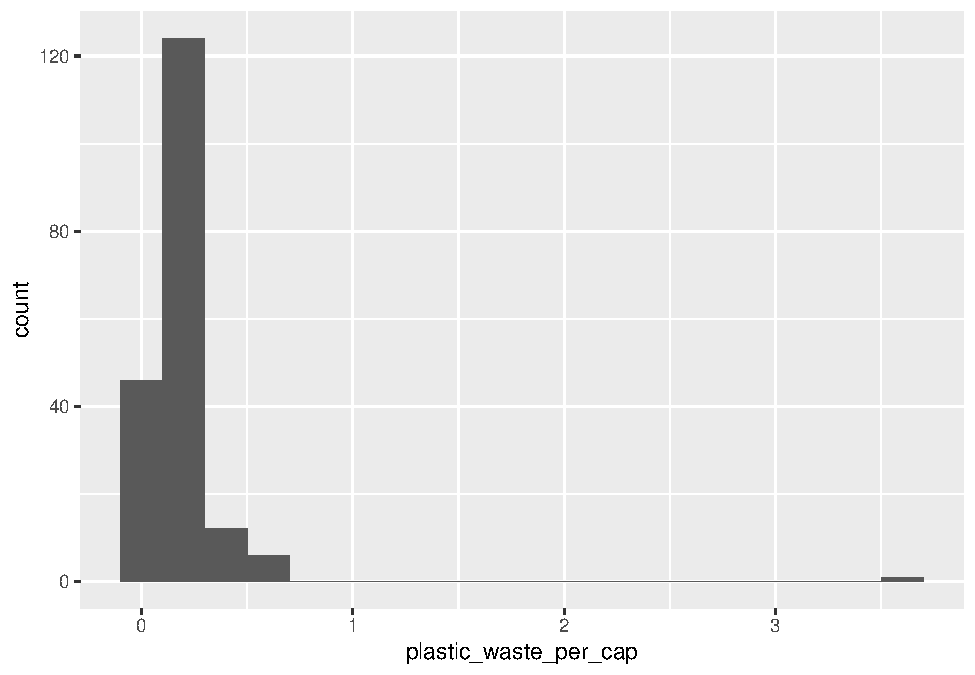
\includegraphics[keepaspectratio]{lab-02-plastic-waste_files/figure-latex/plastic_waste_per_cap-hist-1.pdf}}

One country stands out as an unusual observation at the top of the
distribution. One way of identifying this country is to filter the data
for countries where plastic waste per capita is greater than 3.5
kg/person.

\begin{Shaded}
\begin{Highlighting}[]
\NormalTok{plastic\_waste }\SpecialCharTok{\%\textgreater{}\%}
  \FunctionTok{filter}\NormalTok{(plastic\_waste\_per\_cap }\SpecialCharTok{\textgreater{}} \FloatTok{3.5}\NormalTok{)}
\end{Highlighting}
\end{Shaded}

\begin{verbatim}
## # A tibble: 1 x 10
##   code  entity              continent     year gdp_per_cap plastic_waste_per_cap
##   <chr> <chr>               <chr>        <dbl>       <dbl>                 <dbl>
## 1 TTO   Trinidad and Tobago North Ameri~  2010      31261.                   3.6
## # i 4 more variables: mismanaged_plastic_waste_per_cap <dbl>,
## #   mismanaged_plastic_waste <dbl>, coastal_pop <dbl>, total_pop <dbl>
\end{verbatim}

Did you expect this result? You might consider doing some research on
Trinidad and Tobago to see why plastic waste per capita is so high
there, or whether this is a data error.

The country commonly flagged here is \textbf{Trinidad and Tobago}. High
per-capita values can occur in smaller, high-income, import-dependent
nations with concentrated urban/coastal populations, limited domestic
recycling infrastructure, or sectoral mixes that elevate plastic
throughput. Outliers warrant domain checks (methods, definitions,
population denominators), but this particular spike has been noted in
past compilations.

\subsection{1) Distribution of plastic waste per capita
(2010)}\label{distribution-of-plastic-waste-per-capita-2010}

Plot, using histograms, the distribution of plastic waste per capita
faceted by continent. What can you say about how the continents compare
to each other in terms of their plastic waste per capita?

\begin{Shaded}
\begin{Highlighting}[]
\NormalTok{**NOTE:** From this point onwards the plots and the output of the code are not displayed in the lab instructions, but you can and should the code and view the results yourself.}
\end{Highlighting}
\end{Shaded}

\begin{Shaded}
\begin{Highlighting}[]
\NormalTok{pw\_2010 }\OtherTok{\textless{}{-}}\NormalTok{ plastic\_waste }\SpecialCharTok{\%\textgreater{}\%} \FunctionTok{filter}\NormalTok{(year }\SpecialCharTok{==} \DecValTok{2010}\NormalTok{)}
\end{Highlighting}
\end{Shaded}

\begin{Shaded}
\begin{Highlighting}[]
\FunctionTok{ggplot}\NormalTok{(pw\_2010, }\FunctionTok{aes}\NormalTok{(}\AttributeTok{x =}\NormalTok{ plastic\_waste\_per\_cap)) }\SpecialCharTok{+}
  \FunctionTok{geom\_histogram}\NormalTok{(}\AttributeTok{binwidth =} \FloatTok{0.2}\NormalTok{, }\AttributeTok{boundary =} \DecValTok{0}\NormalTok{, }\AttributeTok{closed =} \StringTok{"left"}\NormalTok{, }\AttributeTok{na.rm =} \ConstantTok{TRUE}\NormalTok{) }\SpecialCharTok{+}
  \FunctionTok{labs}\NormalTok{(}
    \AttributeTok{x =} \StringTok{"Plastic waste per capita (kg/day)"}\NormalTok{,}
    \AttributeTok{y =} \StringTok{"Countries"}\NormalTok{,}
    \AttributeTok{title =} \StringTok{"Distribution of per{-}capita plastic waste (2010)"}
\NormalTok{  )}
\end{Highlighting}
\end{Shaded}

\pandocbounded{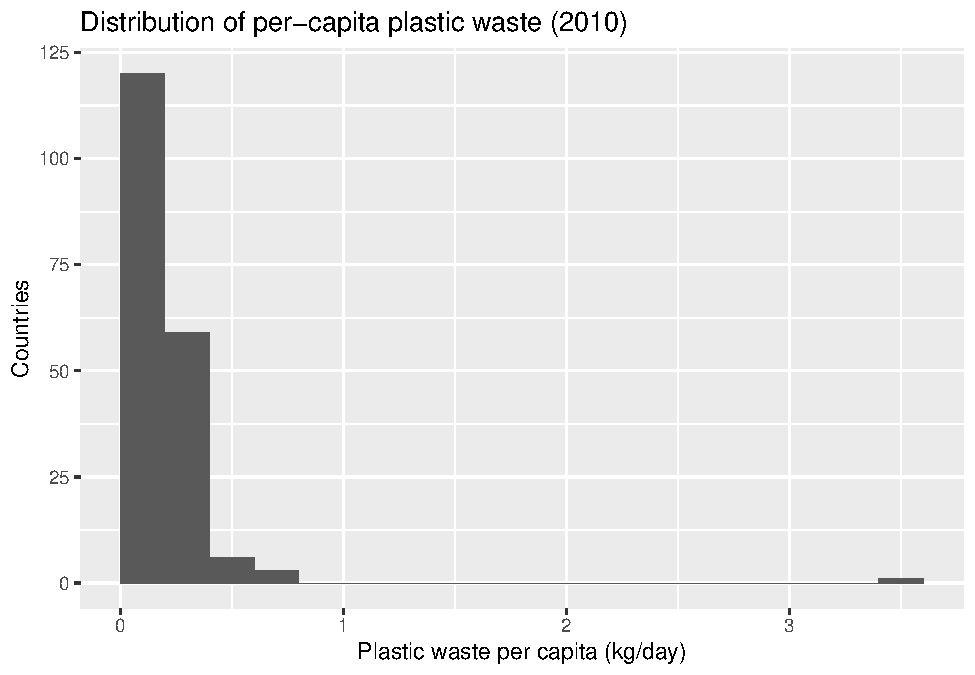
\includegraphics[keepaspectratio]{lab-02-plastic-waste_files/figure-latex/plastic_waste_per_cap-hist-labelled-1.pdf}}

\textbf{Identify the unusually high value (\textgreater{} 3.5 kg/day).}

\begin{Shaded}
\begin{Highlighting}[]
\NormalTok{pw\_2010 }\SpecialCharTok{\%\textgreater{}\%}
  \FunctionTok{filter}\NormalTok{(plastic\_waste\_per\_cap }\SpecialCharTok{\textgreater{}} \FloatTok{3.5}\NormalTok{) }\SpecialCharTok{\%\textgreater{}\%}
  \FunctionTok{arrange}\NormalTok{(}\FunctionTok{desc}\NormalTok{(plastic\_waste\_per\_cap)) }\SpecialCharTok{\%\textgreater{}\%}
  \FunctionTok{select}\NormalTok{(entity, continent, plastic\_waste\_per\_cap)}
\end{Highlighting}
\end{Shaded}

\begin{verbatim}
## # A tibble: 1 x 3
##   entity              continent     plastic_waste_per_cap
##   <chr>               <chr>                         <dbl>
## 1 Trinidad and Tobago North America                   3.6
\end{verbatim}

\subsubsection{Histograms faceted by
continent}\label{histograms-faceted-by-continent}

\begin{Shaded}
\begin{Highlighting}[]
\FunctionTok{ggplot}\NormalTok{(pw\_2010, }\FunctionTok{aes}\NormalTok{(}\AttributeTok{x =}\NormalTok{ plastic\_waste\_per\_cap)) }\SpecialCharTok{+}
  \FunctionTok{geom\_histogram}\NormalTok{(}\AttributeTok{binwidth =} \FloatTok{0.2}\NormalTok{, }\AttributeTok{boundary =} \DecValTok{0}\NormalTok{, }\AttributeTok{closed =} \StringTok{"left"}\NormalTok{, }\AttributeTok{na.rm =} \ConstantTok{TRUE}\NormalTok{) }\SpecialCharTok{+}
  \FunctionTok{facet\_wrap}\NormalTok{(}\SpecialCharTok{\textasciitilde{}}\NormalTok{continent, }\AttributeTok{ncol =} \DecValTok{3}\NormalTok{, }\AttributeTok{scales =} \StringTok{"free\_y"}\NormalTok{) }\SpecialCharTok{+}
  \FunctionTok{labs}\NormalTok{(}
    \AttributeTok{x =} \StringTok{"Plastic waste per capita (kg/day)"}\NormalTok{,}
    \AttributeTok{y =} \StringTok{"Countries"}\NormalTok{,}
    \AttributeTok{title =} \StringTok{"Per{-}capita plastic waste by continent (2010)"}
\NormalTok{  )}
\end{Highlighting}
\end{Shaded}

\pandocbounded{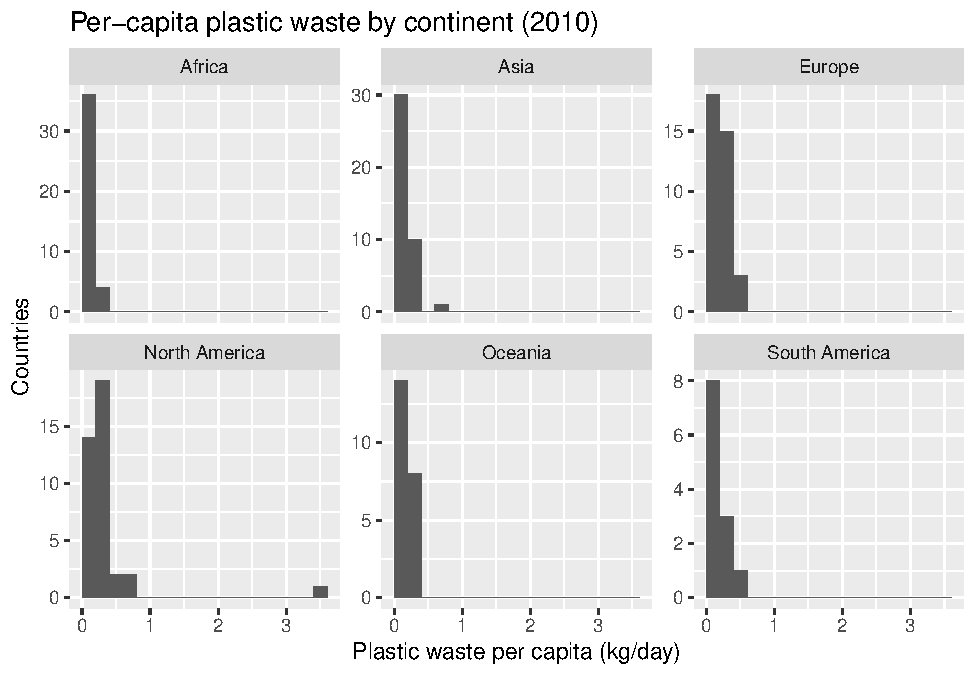
\includegraphics[keepaspectratio]{lab-02-plastic-waste_files/figure-latex/hist-faceted-1.pdf}}

\textbf{Interpretation (succinct, comparative):}

\begin{itemize}
\tightlist
\item
  The \textbf{bulk} of countries in most continents cluster
  \textbf{below \textasciitilde1 kg/day} with \textbf{right-skewed}
  tails.
\item
  Some regions show \textbf{heavier tails} (more countries above
  \textasciitilde1.5 kg/day), highlighting higher consumption and/or
  packaging intensity.
\item
  \texttt{scales\ =\ "free\_y"} avoids continents with more countries
  dominating by raw count and clarifies shape differences.
\end{itemize}

Another way of visualizing numerical data is using density plots.

\begin{Shaded}
\begin{Highlighting}[]
\FunctionTok{ggplot}\NormalTok{(}\AttributeTok{data =}\NormalTok{ plastic\_waste, }\FunctionTok{aes}\NormalTok{(}\AttributeTok{x =}\NormalTok{ plastic\_waste\_per\_cap)) }\SpecialCharTok{+}
  \FunctionTok{geom\_density}\NormalTok{()}
\end{Highlighting}
\end{Shaded}

And compare distributions across continents by colouring density curves
by continent.

\begin{Shaded}
\begin{Highlighting}[]
\FunctionTok{ggplot}\NormalTok{(}
  \AttributeTok{data =}\NormalTok{ plastic\_waste,}
  \AttributeTok{mapping =} \FunctionTok{aes}\NormalTok{(}
    \AttributeTok{x =}\NormalTok{ plastic\_waste\_per\_cap,}
    \AttributeTok{color =}\NormalTok{ continent}
\NormalTok{  )}
\NormalTok{) }\SpecialCharTok{+}
  \FunctionTok{geom\_density}\NormalTok{()}
\end{Highlighting}
\end{Shaded}

The resulting plot may be a little difficult to read, so let's also fill
the curves in with colours as well.

\begin{Shaded}
\begin{Highlighting}[]
\FunctionTok{ggplot}\NormalTok{(}
  \AttributeTok{data =}\NormalTok{ plastic\_waste,}
  \AttributeTok{mapping =} \FunctionTok{aes}\NormalTok{(}
    \AttributeTok{x =}\NormalTok{ plastic\_waste\_per\_cap,}
    \AttributeTok{color =}\NormalTok{ continent,}
    \AttributeTok{fill =}\NormalTok{ continent}
\NormalTok{  )}
\NormalTok{) }\SpecialCharTok{+}
  \FunctionTok{geom\_density}\NormalTok{()}
\end{Highlighting}
\end{Shaded}

The overlapping colours make it difficult to tell what's happening with
the distributions in continents plotted first, and hence covered by
continents plotted over them. We can change the transparency level of
the fill color to help with this. The \texttt{alpha} argument takes
values between 0 and 1: 0 is completely transparent and 1 is completely
opaque. There is no way to tell what value will work best, so you just
need to try a few.

\begin{Shaded}
\begin{Highlighting}[]
\FunctionTok{ggplot}\NormalTok{(}
  \AttributeTok{data =}\NormalTok{ plastic\_waste,}
  \AttributeTok{mapping =} \FunctionTok{aes}\NormalTok{(}
    \AttributeTok{x =}\NormalTok{ plastic\_waste\_per\_cap,}
    \AttributeTok{color =}\NormalTok{ continent,}
    \AttributeTok{fill =}\NormalTok{ continent}
\NormalTok{  )}
\NormalTok{) }\SpecialCharTok{+}
  \FunctionTok{geom\_density}\NormalTok{(}\AttributeTok{alpha =} \FloatTok{0.7}\NormalTok{)}
\end{Highlighting}
\end{Shaded}

This still doesn't look great\ldots{}

\begin{enumerate}
\def\labelenumi{\arabic{enumi}.}
\item
  Recreate the density plots above using a different (lower) alpha level
  that works better for displaying the density curves for all
  continents.
\item
  Describe why we defined the \texttt{color} and \texttt{fill} of the
  curves by mapping aesthetics of the plot but we defined the
  \texttt{alpha} level as a characteristic of the plotting geom.
\end{enumerate}

\subsection{2) Density plots (global \& by continent) and
transparency}\label{density-plots-global-by-continent-and-transparency}

\begin{Shaded}
\begin{Highlighting}[]
\FunctionTok{ggplot}\NormalTok{(pw\_2010, }\FunctionTok{aes}\NormalTok{(}\AttributeTok{x =}\NormalTok{ plastic\_waste\_per\_cap)) }\SpecialCharTok{+}
  \FunctionTok{geom\_density}\NormalTok{(}\AttributeTok{na.rm =} \ConstantTok{TRUE}\NormalTok{) }\SpecialCharTok{+}
  \FunctionTok{labs}\NormalTok{(}
    \AttributeTok{x =} \StringTok{"Plastic waste per capita (kg/day)"}\NormalTok{, }\AttributeTok{y =} \StringTok{"Density"}\NormalTok{,}
    \AttributeTok{title =} \StringTok{"Global density of per{-}capita plastic waste (2010)"}
\NormalTok{  )}
\end{Highlighting}
\end{Shaded}

\pandocbounded{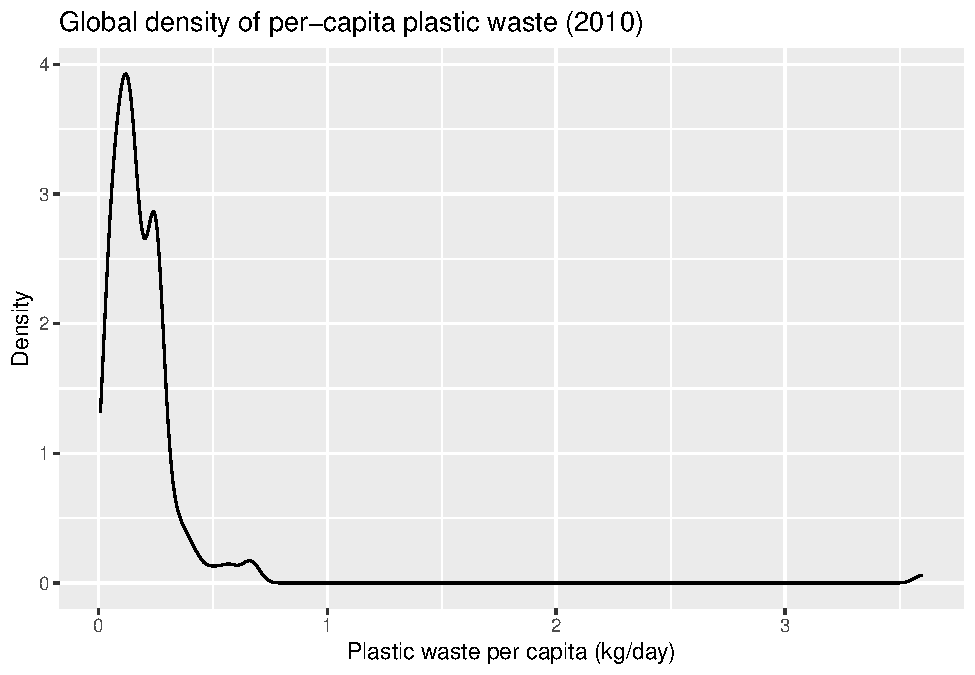
\includegraphics[keepaspectratio]{lab-02-plastic-waste_files/figure-latex/dens-global-1.pdf}}

\begin{Shaded}
\begin{Highlighting}[]
\FunctionTok{ggplot}\NormalTok{(pw\_2010, }\FunctionTok{aes}\NormalTok{(}\AttributeTok{x =}\NormalTok{ plastic\_waste\_per\_cap, }\AttributeTok{color =}\NormalTok{ continent)) }\SpecialCharTok{+}
  \FunctionTok{geom\_density}\NormalTok{(}\AttributeTok{na.rm =} \ConstantTok{TRUE}\NormalTok{) }\SpecialCharTok{+}
  \FunctionTok{labs}\NormalTok{(}\AttributeTok{x =} \StringTok{"Plastic waste per capita (kg/day)"}\NormalTok{, }\AttributeTok{y =} \StringTok{"Density"}\NormalTok{, }\AttributeTok{color =} \StringTok{"Continent"}\NormalTok{)}
\end{Highlighting}
\end{Shaded}

\pandocbounded{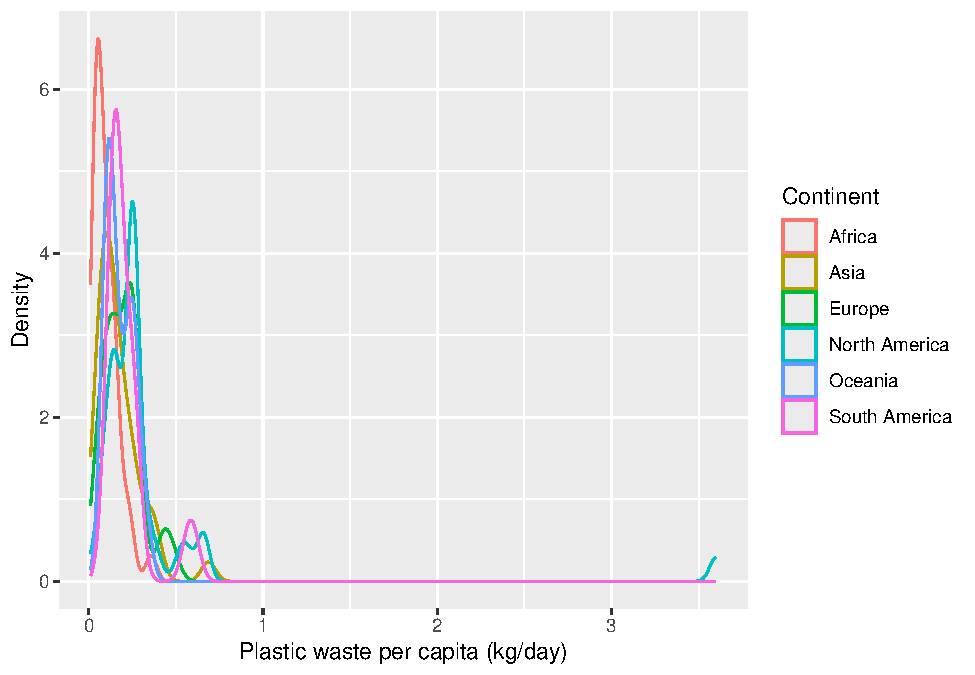
\includegraphics[keepaspectratio]{lab-02-plastic-waste_files/figure-latex/dens-by-continent-outline-1.pdf}}

\begin{Shaded}
\begin{Highlighting}[]
\FunctionTok{ggplot}\NormalTok{(pw\_2010, }\FunctionTok{aes}\NormalTok{(}\AttributeTok{x =}\NormalTok{ plastic\_waste\_per\_cap, }\AttributeTok{color =}\NormalTok{ continent, }\AttributeTok{fill =}\NormalTok{ continent)) }\SpecialCharTok{+}
  \FunctionTok{geom\_density}\NormalTok{(}\AttributeTok{alpha =} \FloatTok{0.05}\NormalTok{, }\AttributeTok{na.rm =} \ConstantTok{TRUE}\NormalTok{) }\SpecialCharTok{+}
  \FunctionTok{labs}\NormalTok{(}\AttributeTok{x =} \StringTok{"Plastic waste per capita (kg/day)"}\NormalTok{, }\AttributeTok{y =} \StringTok{"Density"}\NormalTok{, }\AttributeTok{color =} \StringTok{"Continent"}\NormalTok{, }\AttributeTok{fill =} \StringTok{"Continent"}\NormalTok{)}
\end{Highlighting}
\end{Shaded}

\pandocbounded{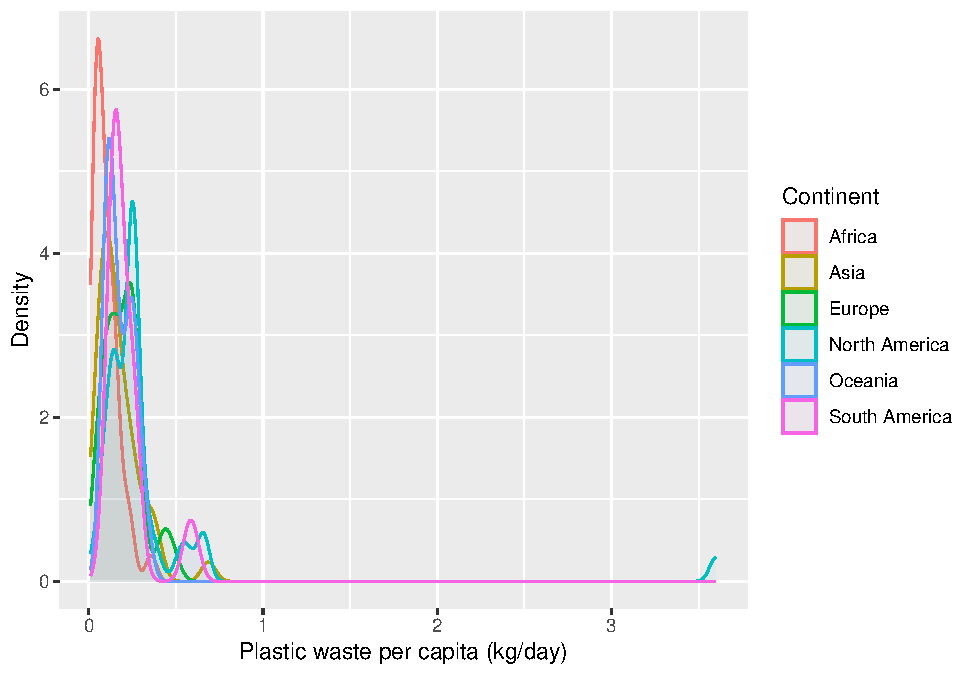
\includegraphics[keepaspectratio]{lab-02-plastic-waste_files/figure-latex/dens-by-continent-fill-alpha-1.pdf}}

\textbf{Why are \texttt{color} and \texttt{fill} mapped but
\texttt{alpha} is given as a geom argument?}\\

\texttt{color} and \texttt{fill} represent \textbf{data-driven
aesthetics}---in this case, the continent varies from row to row, so
each observation needs to be assigned a different colour or fill based
on its group. That makes them part of the aesthetic mapping, defined
inside \texttt{aes()}.

By contrast, \texttt{alpha} is used here as a \textbf{constant styling
choice}, applied the same way to all groups to improve readability of
overlapping densities. Since it is not tied to any variable in the
dataset, it is specified directly in the geom (outside \texttt{aes})
rather than mapped to the data. If we wanted transparency itself to vary
by a data column, only then would we place \texttt{alpha} inside
\texttt{aes()}.

🧶 ✅ ⬆️ \emph{Now is a good time to knit your document and commit and
push your changes to GitHub with an appropriate commit message. Make
sure to commit and push all changed files so that your Git pane is
cleared up afterwards.}

And yet another way to visualize this relationship is using side-by-side
box plots.

\begin{Shaded}
\begin{Highlighting}[]
\FunctionTok{ggplot}\NormalTok{(}
  \AttributeTok{data =}\NormalTok{ plastic\_waste,}
  \AttributeTok{mapping =} \FunctionTok{aes}\NormalTok{(}
    \AttributeTok{x =}\NormalTok{ continent,}
    \AttributeTok{y =}\NormalTok{ plastic\_waste\_per\_cap}
\NormalTok{  )}
\NormalTok{) }\SpecialCharTok{+}
  \FunctionTok{geom\_boxplot}\NormalTok{()}
\end{Highlighting}
\end{Shaded}

Convert your side-by-side box plots from the previous task to
\href{http://ggplot2.tidyverse.org/reference/geom_violin.html}{violin
plots}. What do the violin plots reveal that box plots do not? What
features are apparent in the box plots but not in the violin plots?

\subsection{4) Side-by-side box plots → violin
plots}\label{side-by-side-box-plots-violin-plots}

\begin{Shaded}
\begin{Highlighting}[]
\FunctionTok{ggplot}\NormalTok{(pw\_2010, }\FunctionTok{aes}\NormalTok{(}\AttributeTok{x =}\NormalTok{ continent, }\AttributeTok{y =}\NormalTok{ plastic\_waste\_per\_cap)) }\SpecialCharTok{+}
  \FunctionTok{geom\_boxplot}\NormalTok{(}\AttributeTok{na.rm =} \ConstantTok{TRUE}\NormalTok{, }\AttributeTok{outlier.alpha =} \FloatTok{0.8}\NormalTok{) }\SpecialCharTok{+}
  \FunctionTok{labs}\NormalTok{(}
    \AttributeTok{x =} \StringTok{"Continent"}\NormalTok{, }\AttributeTok{y =} \StringTok{"Plastic waste per capita (kg/day)"}\NormalTok{,}
    \AttributeTok{title =} \StringTok{"Per{-}capita plastic waste by continent — box plots"}
\NormalTok{  )}
\end{Highlighting}
\end{Shaded}

\begin{verbatim}
## Warning in grid.Call(C_textBounds, as.graphicsAnnot(x$label), x$x, x$y, :
## conversion failure on 'Per-capita plastic waste by continent — box plots' in
## 'mbcsToSbcs': dot substituted for <e2>
\end{verbatim}

\begin{verbatim}
## Warning in grid.Call(C_textBounds, as.graphicsAnnot(x$label), x$x, x$y, :
## conversion failure on 'Per-capita plastic waste by continent — box plots' in
## 'mbcsToSbcs': dot substituted for <80>
\end{verbatim}

\begin{verbatim}
## Warning in grid.Call(C_textBounds, as.graphicsAnnot(x$label), x$x, x$y, :
## conversion failure on 'Per-capita plastic waste by continent — box plots' in
## 'mbcsToSbcs': dot substituted for <94>
\end{verbatim}

\begin{verbatim}
## Warning in grid.Call.graphics(C_text, as.graphicsAnnot(x$label), x$x, x$y, :
## conversion failure on 'Per-capita plastic waste by continent — box plots' in
## 'mbcsToSbcs': dot substituted for <e2>
\end{verbatim}

\begin{verbatim}
## Warning in grid.Call.graphics(C_text, as.graphicsAnnot(x$label), x$x, x$y, :
## conversion failure on 'Per-capita plastic waste by continent — box plots' in
## 'mbcsToSbcs': dot substituted for <80>
\end{verbatim}

\begin{verbatim}
## Warning in grid.Call.graphics(C_text, as.graphicsAnnot(x$label), x$x, x$y, :
## conversion failure on 'Per-capita plastic waste by continent — box plots' in
## 'mbcsToSbcs': dot substituted for <94>
\end{verbatim}

\pandocbounded{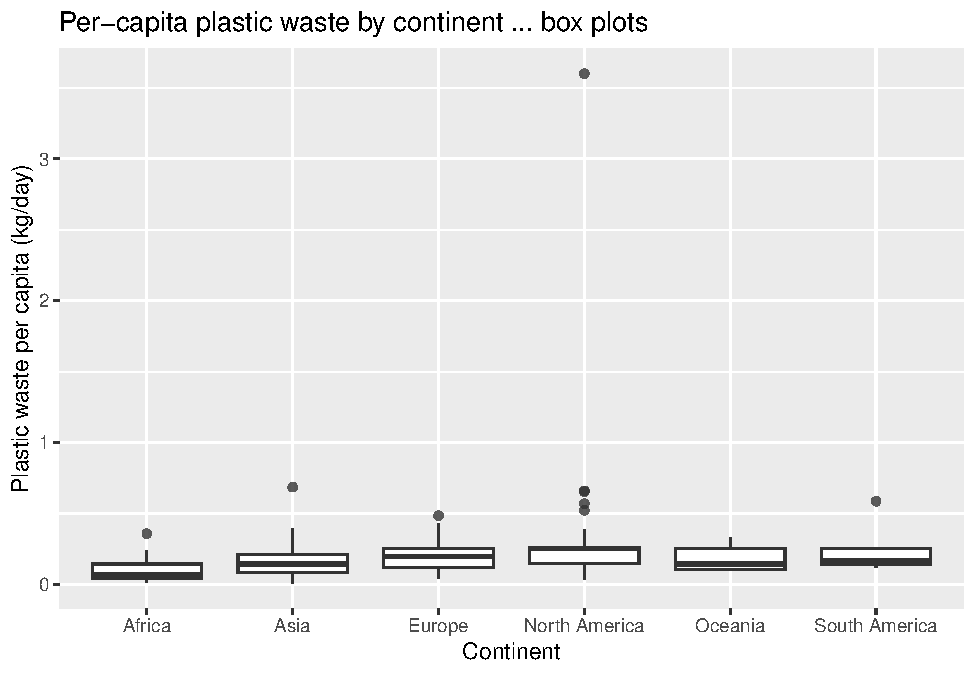
\includegraphics[keepaspectratio]{lab-02-plastic-waste_files/figure-latex/boxplots-1.pdf}}

\begin{Shaded}
\begin{Highlighting}[]
\FunctionTok{ggplot}\NormalTok{(pw\_2010, }\FunctionTok{aes}\NormalTok{(}\AttributeTok{x =}\NormalTok{ continent, }\AttributeTok{y =}\NormalTok{ plastic\_waste\_per\_cap)) }\SpecialCharTok{+}
  \FunctionTok{geom\_violin}\NormalTok{(}\AttributeTok{trim =} \ConstantTok{FALSE}\NormalTok{, }\AttributeTok{na.rm =} \ConstantTok{TRUE}\NormalTok{) }\SpecialCharTok{+}
  \FunctionTok{stat\_summary}\NormalTok{(}\AttributeTok{fun =}\NormalTok{ median, }\AttributeTok{geom =} \StringTok{"point"}\NormalTok{, }\AttributeTok{size =} \FloatTok{1.7}\NormalTok{, }\AttributeTok{na.rm =} \ConstantTok{TRUE}\NormalTok{) }\SpecialCharTok{+}
  \FunctionTok{labs}\NormalTok{(}
    \AttributeTok{x =} \StringTok{"Continent"}\NormalTok{, }\AttributeTok{y =} \StringTok{"Plastic waste per capita (kg/day)"}\NormalTok{,}
    \AttributeTok{title =} \StringTok{"Per{-}capita plastic waste by continent — violins with medians"}
\NormalTok{  )}
\end{Highlighting}
\end{Shaded}

\begin{verbatim}
## Warning in grid.Call(C_textBounds, as.graphicsAnnot(x$label), x$x, x$y, :
## conversion failure on 'Per-capita plastic waste by continent — violins with
## medians' in 'mbcsToSbcs': dot substituted for <e2>
\end{verbatim}

\begin{verbatim}
## Warning in grid.Call(C_textBounds, as.graphicsAnnot(x$label), x$x, x$y, :
## conversion failure on 'Per-capita plastic waste by continent — violins with
## medians' in 'mbcsToSbcs': dot substituted for <80>
\end{verbatim}

\begin{verbatim}
## Warning in grid.Call(C_textBounds, as.graphicsAnnot(x$label), x$x, x$y, :
## conversion failure on 'Per-capita plastic waste by continent — violins with
## medians' in 'mbcsToSbcs': dot substituted for <94>
\end{verbatim}

\begin{verbatim}
## Warning in grid.Call.graphics(C_text, as.graphicsAnnot(x$label), x$x, x$y, :
## conversion failure on 'Per-capita plastic waste by continent — violins with
## medians' in 'mbcsToSbcs': dot substituted for <e2>
\end{verbatim}

\begin{verbatim}
## Warning in grid.Call.graphics(C_text, as.graphicsAnnot(x$label), x$x, x$y, :
## conversion failure on 'Per-capita plastic waste by continent — violins with
## medians' in 'mbcsToSbcs': dot substituted for <80>
\end{verbatim}

\begin{verbatim}
## Warning in grid.Call.graphics(C_text, as.graphicsAnnot(x$label), x$x, x$y, :
## conversion failure on 'Per-capita plastic waste by continent — violins with
## medians' in 'mbcsToSbcs': dot substituted for <94>
\end{verbatim}

\pandocbounded{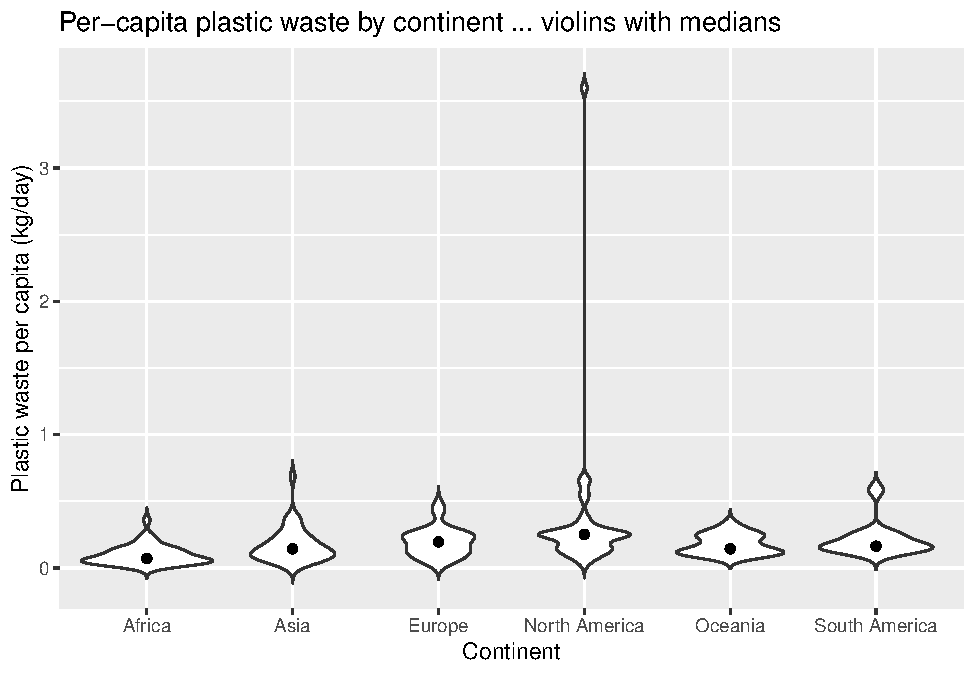
\includegraphics[keepaspectratio]{lab-02-plastic-waste_files/figure-latex/violins-1.pdf}}

\textbf{Compare:}

\begin{itemize}
\item
  \textbf{Violins reveal shape (multi-modality, tail thickness) hidden
  by box plots.} They show the full distribution, making patterns like
  multiple peaks, skewness, or dense clusters more visible.
\item
  \textbf{Box plots emphasize median, IQR, and conventional outliers;
  clearer for compact comparisons across groups.} They simplify
  distributions into key summaries, making it easy to compare central
  tendency and spread side by side.
\item
  \textbf{Using both offers complementary insight: use violins to see
  structure; box plots to summarize.} Together they provide both the
  detail of distributional shape and the clarity of statistical
  landmarks.
\end{itemize}

\subsection{5) Mismanaged vs per-capita plastic waste
(scatter)}\label{mismanaged-vs-per-capita-plastic-waste-scatter}

Visualize the relationship between plastic waste per capita and
mismanaged plastic waste per capita using a scatterplot. Describe the
relationship.

\begin{Shaded}
\begin{Highlighting}[]
\FunctionTok{ggplot}\NormalTok{(pw\_2010, }\FunctionTok{aes}\NormalTok{(}\AttributeTok{x =}\NormalTok{ plastic\_waste\_per\_cap, }\AttributeTok{y =}\NormalTok{ mismanaged\_plastic\_waste\_per\_cap)) }\SpecialCharTok{+}
  \FunctionTok{geom\_point}\NormalTok{(}\AttributeTok{na.rm =} \ConstantTok{TRUE}\NormalTok{) }\SpecialCharTok{+}
  \FunctionTok{labs}\NormalTok{(}
    \AttributeTok{x =} \StringTok{"Plastic waste per capita (kg/day)"}\NormalTok{,}
    \AttributeTok{y =} \StringTok{"Mismanaged plastic waste per capita (kg/day)"}\NormalTok{,}
    \AttributeTok{title =} \StringTok{"Mismanaged vs total per{-}capita plastic waste (2010)"}
\NormalTok{  )}
\end{Highlighting}
\end{Shaded}

\pandocbounded{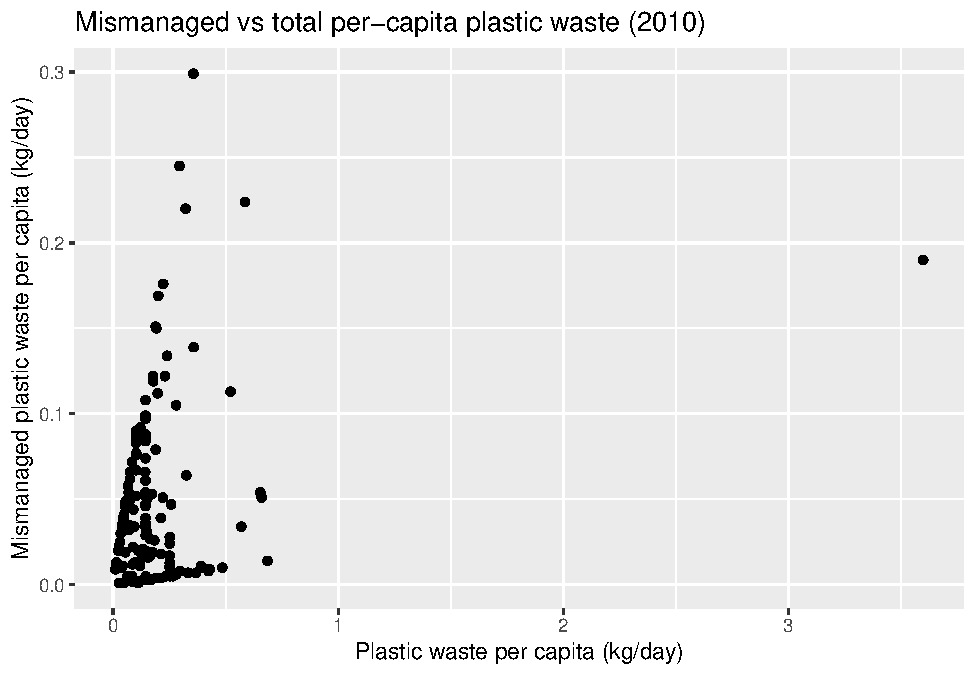
\includegraphics[keepaspectratio]{lab-02-plastic-waste_files/figure-latex/mismanaged-vs-pw-1.pdf}}

\textbf{Relationship (direct):} The relationship is generally
\textbf{positive}: countries that generate more plastic waste per person
also tend to mismanage a larger amount of waste per person. However, the
\textbf{wide spread of points} reveals substantial variation in
outcomes. Some nations manage to keep mismanaged waste relatively low
despite high per-capita generation, likely reflecting stronger
collection and recycling systems, while others mismanage
disproportionately large amounts even at moderate generation levels.
This heterogeneity underscores that \textbf{waste-management efficiency
and infrastructure quality} play a critical role in shaping outcomes
beyond simple generation rates.

\textbf{Colour by continent}

Colour the points in the scatterplot by continent. Does there seem to be
any clear distinctions between continents with respect to how plastic
waste per capita and mismanaged plastic waste per capita are associated?

\begin{Shaded}
\begin{Highlighting}[]
\FunctionTok{ggplot}\NormalTok{(pw\_2010, }\FunctionTok{aes}\NormalTok{(}\AttributeTok{x =}\NormalTok{ plastic\_waste\_per\_cap, }\AttributeTok{y =}\NormalTok{ mismanaged\_plastic\_waste\_per\_cap, }\AttributeTok{color =}\NormalTok{ continent)) }\SpecialCharTok{+}
  \FunctionTok{geom\_point}\NormalTok{(}\AttributeTok{na.rm =} \ConstantTok{TRUE}\NormalTok{) }\SpecialCharTok{+}
  \FunctionTok{labs}\NormalTok{(}
    \AttributeTok{x =} \StringTok{"Plastic waste per capita (kg/day)"}\NormalTok{,}
    \AttributeTok{y =} \StringTok{"Mismanaged plastic waste per capita (kg/day)"}\NormalTok{,}
    \AttributeTok{color =} \StringTok{"Continent"}\NormalTok{,}
    \AttributeTok{title =} \StringTok{"Mismanaged vs total per{-}capita plastic waste by continent (2010)"}
\NormalTok{  )}
\end{Highlighting}
\end{Shaded}

\pandocbounded{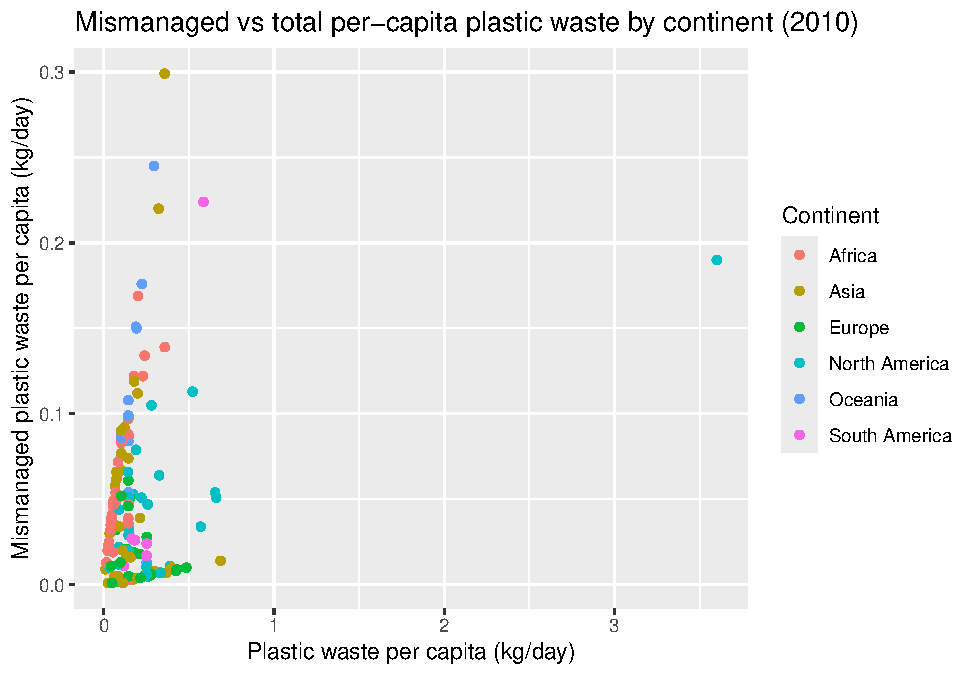
\includegraphics[keepaspectratio]{lab-02-plastic-waste_files/figure-latex/mismanaged-vs-pw-continent-1.pdf}}

\textbf{Added insight:} Continental clusters suggest \textbf{regional
infrastructure and policy} differences: some regions show similar
per-capita generation but \textbf{lower mismanagement}, pointing to
better collection/recycling systems.

\subsection{6) Per-capita waste vs population (total \&
coastal)}\label{per-capita-waste-vs-population-total-coastal}

Visualize the relationship between plastic waste per capita and total
population as well as plastic waste per capita and coastal population.
You will need to make two separate plots. Do either of these pairs of
variables appear to be more strongly linearly associated?

\begin{Shaded}
\begin{Highlighting}[]
\FunctionTok{ggplot}\NormalTok{(pw\_2010, }\FunctionTok{aes}\NormalTok{(}\AttributeTok{x =}\NormalTok{ total\_pop, }\AttributeTok{y =}\NormalTok{ plastic\_waste\_per\_cap)) }\SpecialCharTok{+}
  \FunctionTok{geom\_point}\NormalTok{(}\AttributeTok{na.rm =} \ConstantTok{TRUE}\NormalTok{) }\SpecialCharTok{+}
  \FunctionTok{scale\_x\_log10}\NormalTok{(}\AttributeTok{labels =} \FunctionTok{label\_number}\NormalTok{()) }\SpecialCharTok{+}
  \FunctionTok{labs}\NormalTok{(}
    \AttributeTok{x =} \StringTok{"Total population (log10, SI)"}\NormalTok{, }\AttributeTok{y =} \StringTok{"Plastic waste per capita (kg/day)"}\NormalTok{,}
    \AttributeTok{title =} \StringTok{"Per{-}capita plastic waste vs total population"}
\NormalTok{  )}
\end{Highlighting}
\end{Shaded}

\pandocbounded{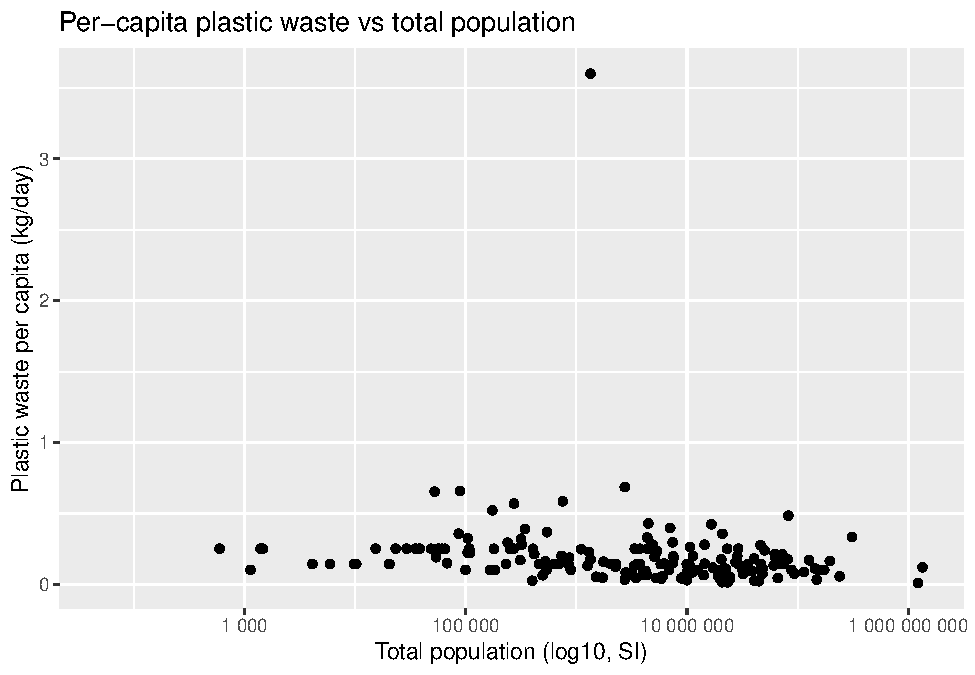
\includegraphics[keepaspectratio]{lab-02-plastic-waste_files/figure-latex/pw-vs-totalpop-1.pdf}}

\begin{Shaded}
\begin{Highlighting}[]
\FunctionTok{ggplot}\NormalTok{(pw\_2010, }\FunctionTok{aes}\NormalTok{(}\AttributeTok{x =}\NormalTok{ coastal\_pop, }\AttributeTok{y =}\NormalTok{ plastic\_waste\_per\_cap)) }\SpecialCharTok{+}
  \FunctionTok{geom\_point}\NormalTok{(}\AttributeTok{na.rm =} \ConstantTok{TRUE}\NormalTok{) }\SpecialCharTok{+}
  \FunctionTok{scale\_x\_log10}\NormalTok{(}\AttributeTok{labels =} \FunctionTok{label\_number}\NormalTok{()) }\SpecialCharTok{+}
  \FunctionTok{labs}\NormalTok{(}
    \AttributeTok{x =} \StringTok{"Coastal population (log10, SI)"}\NormalTok{, }\AttributeTok{y =} \StringTok{"Plastic waste per capita (kg/day)"}\NormalTok{,}
    \AttributeTok{title =} \StringTok{"Per{-}capita plastic waste vs coastal population"}
\NormalTok{  )}
\end{Highlighting}
\end{Shaded}

\pandocbounded{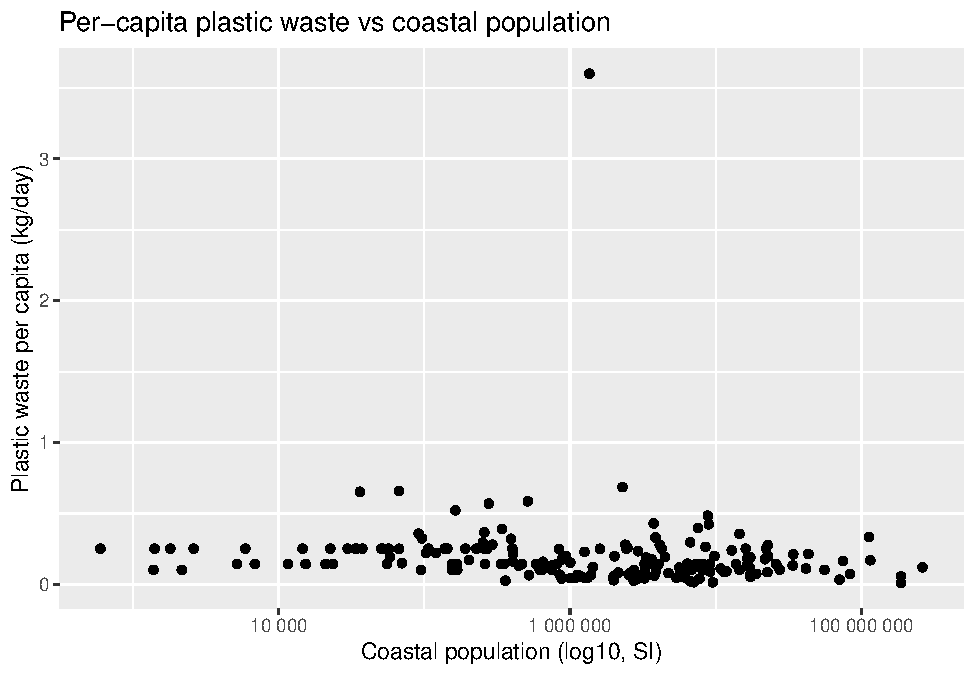
\includegraphics[keepaspectratio]{lab-02-plastic-waste_files/figure-latex/pw-vs-coastalpop-1.pdf}}

\textbf{Which appears more linear?} Neither relationship demonstrates a
strong linear pattern. Even after applying a log transformation to
reduce the skew from very large population values, the association
between coastal population and per-capita plastic waste appears only
slightly tighter than that observed with total population. This suggests
that while countries with larger coastal populations may, in some cases,
generate more plastic waste per person, the effect is not consistent or
dominant.

The weakness of the signal indicates that population metrics
alone---whether overall or coastal---are insufficient to explain
variations in per-capita plastic waste. Instead, factors such as
consumption habits, waste-management infrastructure, cultural practices,
levels of industrialization, and the prevalence of single-use plastics
are likely more decisive. Wealthier nations with smaller populations can
produce high per-capita waste due to higher consumption, whereas
large-population countries may generate relatively low per-capita waste
if infrastructure and cultural practices limit plastic usage. Population
size sets the stage for potential waste generation but does not
determine outcomes. It is the interaction of economic, social, and
infrastructural conditions that largely drives the observed differences
in plastic waste per capita across countries.

🧶 ✅ ⬆️ \emph{Now is another good time to knit your document and commit
and push your changes to GitHub with an appropriate commit message. Make
sure to commit and push all changed files so that your Git pane is
cleared up afterwards.}

\section{Wrapping up}\label{wrapping-up}

We don't expect you to complete all of the exercises within the hour
reserved for the live workshop. Ideally, you should have got to this
point. If you still have some time left, move on to the remaining
exercises below. If not, you should find a time to meet with your team
and complete them after the workshop. If you haven't had time to finish
the exercises above, please ask for help before you leave!

\begin{Shaded}
\begin{Highlighting}[]
\NormalTok{**Hint:** The x{-}axis is a calculated variable. One country with plastic waste per capita over 3 kg/day has been filtered out. And the data are not only represented with points on the plot but also a smooth curve. The term "smooth" should help you [pick which geom to use](https://ggplot2.tidyverse.org/reference/index.html\#section{-}geoms).}
\end{Highlighting}
\end{Shaded}

Recreate the following plot, and interpret what you see in context of
the data.

\subsection{7) Recreate and interpret the coastal proportion
plot}\label{recreate-and-interpret-the-coastal-proportion-plot}

\begin{Shaded}
\begin{Highlighting}[]
\NormalTok{pw\_2010 }\SpecialCharTok{\%\textgreater{}\%}
  \FunctionTok{mutate}\NormalTok{(}\AttributeTok{coastal\_pop\_prop =}\NormalTok{ coastal\_pop }\SpecialCharTok{/}\NormalTok{ total\_pop) }\SpecialCharTok{\%\textgreater{}\%}
  \FunctionTok{filter}\NormalTok{(plastic\_waste\_per\_cap }\SpecialCharTok{\textless{}} \DecValTok{3}\NormalTok{) }\SpecialCharTok{\%\textgreater{}\%}
  \FunctionTok{ggplot}\NormalTok{(}\FunctionTok{aes}\NormalTok{(}\AttributeTok{x =}\NormalTok{ coastal\_pop\_prop, }\AttributeTok{y =}\NormalTok{ plastic\_waste\_per\_cap, }\AttributeTok{color =}\NormalTok{ continent)) }\SpecialCharTok{+}
  \FunctionTok{geom\_point}\NormalTok{(}\AttributeTok{na.rm =} \ConstantTok{TRUE}\NormalTok{) }\SpecialCharTok{+}
  \FunctionTok{geom\_smooth}\NormalTok{(}\AttributeTok{color =} \StringTok{"black"}\NormalTok{, }\AttributeTok{se =} \ConstantTok{TRUE}\NormalTok{, }\AttributeTok{na.rm =} \ConstantTok{TRUE}\NormalTok{) }\SpecialCharTok{+}
  \FunctionTok{scale\_color\_viridis\_d}\NormalTok{() }\SpecialCharTok{+}
  \FunctionTok{labs}\NormalTok{(}
    \AttributeTok{x =} \StringTok{"Coastal population proportion (coastal / total)"}\NormalTok{,}
    \AttributeTok{y =} \StringTok{"Plastic waste per capita (kg/day)"}\NormalTok{,}
    \AttributeTok{color =} \StringTok{"Continent"}\NormalTok{,}
    \AttributeTok{title =} \StringTok{"Plastic waste vs coastal population proportion"}\NormalTok{,}
    \AttributeTok{subtitle =} \StringTok{"2010; one extreme per{-}capita country filtered out"}
\NormalTok{  ) }\SpecialCharTok{+}
  \FunctionTok{theme\_minimal}\NormalTok{()}
\end{Highlighting}
\end{Shaded}

\begin{verbatim}
## `geom_smooth()` using method = 'loess' and formula = 'y ~ x'
\end{verbatim}

\pandocbounded{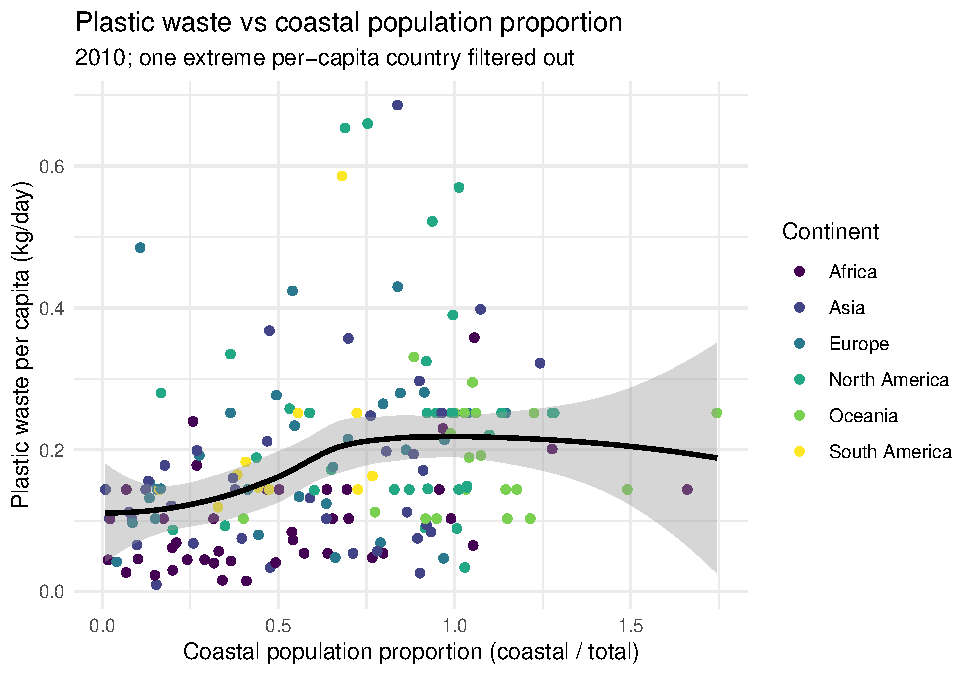
\includegraphics[keepaspectratio]{lab-02-plastic-waste_files/figure-latex/coastal-prop-plot-1.pdf}}

\textbf{Interpretation (in context):}

\begin{itemize}
\tightlist
\item
  The \textbf{black smoothing} line suggests a \textbf{gentle upward
  trend}: nations with a larger share of their population living
  \textbf{along the coast} generally exhibit slightly higher levels of
  per-capita plastic waste.
\item
  Regional colour groupings highlight contrasts: some continents cluster
  at lower coastal proportions with correspondingly lower waste, while
  others extend into higher coastal shares coupled with greater waste
  levels---patterns consistent with \textbf{dense coastal urbanization,
  reliance on imports, and tourism-driven consumption}.
\item
  The \texttt{\textless{}\ 3} filter was applied to prevent a single
  extreme outlier from disproportionately shaping the fitted trend.
\end{itemize}

🧶 ✅ ⬆️ Knit, \emph{commit, and push your changes to GitHub with an
appropriate commit message. Make sure to commit and push all changed
files so that your Git pane is cleared up afterwards and review the md
document on GitHub to make sure you're happy with the final state of
your work.}

Once you're done, check to make sure your latest changes are on GitHub
and that you have a green indicator for the automated check for your R
Markdown document knitting.

\pandocbounded{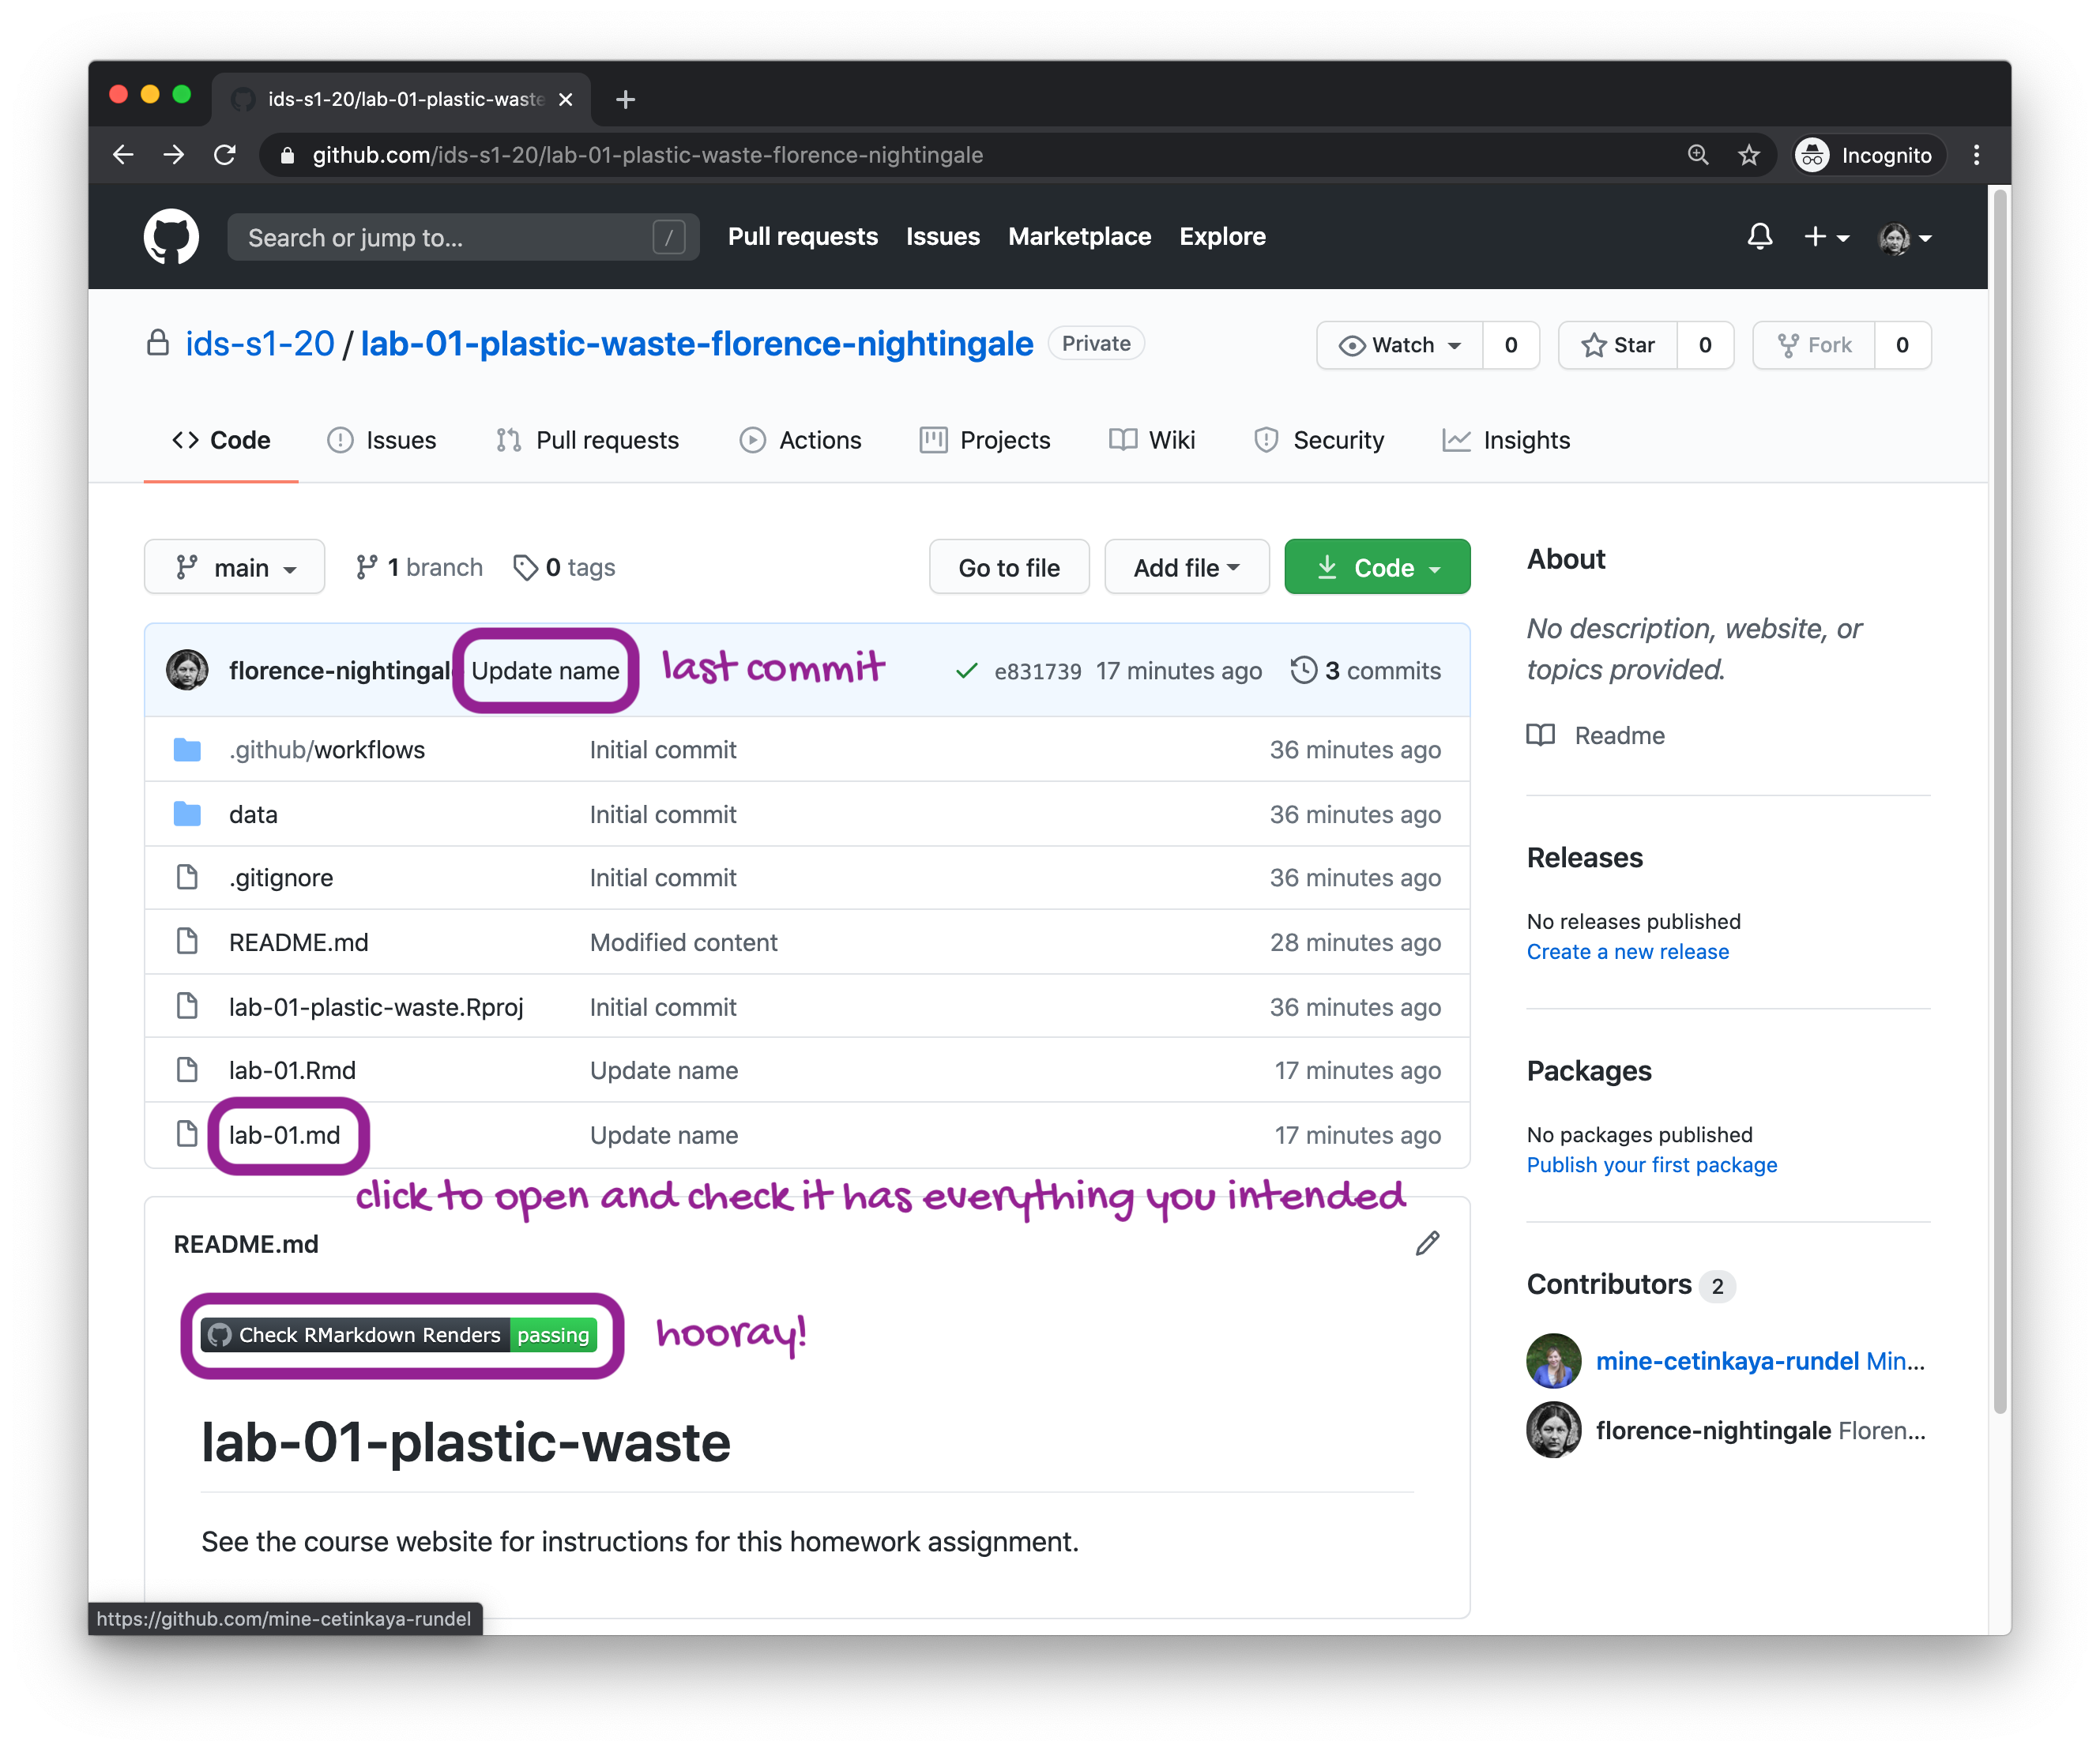
\includegraphics[keepaspectratio]{img/repo-end.png}}

\subsection{8) Summary statistics by continent (concise report
table)}\label{summary-statistics-by-continent-concise-report-table}

\begin{Shaded}
\begin{Highlighting}[]
\NormalTok{pw\_2010 }\SpecialCharTok{\%\textgreater{}\%}
  \FunctionTok{group\_by}\NormalTok{(continent) }\SpecialCharTok{\%\textgreater{}\%}
  \FunctionTok{summarise}\NormalTok{(}
    \AttributeTok{n      =} \FunctionTok{n}\NormalTok{(),}
    \AttributeTok{mean   =} \FunctionTok{mean}\NormalTok{(plastic\_waste\_per\_cap, }\AttributeTok{na.rm =} \ConstantTok{TRUE}\NormalTok{),}
    \AttributeTok{median =} \FunctionTok{median}\NormalTok{(plastic\_waste\_per\_cap, }\AttributeTok{na.rm =} \ConstantTok{TRUE}\NormalTok{),}
    \AttributeTok{sd     =} \FunctionTok{sd}\NormalTok{(plastic\_waste\_per\_cap, }\AttributeTok{na.rm =} \ConstantTok{TRUE}\NormalTok{),}
    \AttributeTok{iqr    =} \FunctionTok{IQR}\NormalTok{(plastic\_waste\_per\_cap, }\AttributeTok{na.rm =} \ConstantTok{TRUE}\NormalTok{),}
    \AttributeTok{min    =} \FunctionTok{min}\NormalTok{(plastic\_waste\_per\_cap, }\AttributeTok{na.rm =} \ConstantTok{TRUE}\NormalTok{),}
    \AttributeTok{max    =} \FunctionTok{max}\NormalTok{(plastic\_waste\_per\_cap, }\AttributeTok{na.rm =} \ConstantTok{TRUE}\NormalTok{)}
\NormalTok{  ) }\SpecialCharTok{\%\textgreater{}\%}
  \FunctionTok{arrange}\NormalTok{(}\FunctionTok{desc}\NormalTok{(median))}
\end{Highlighting}
\end{Shaded}

\begin{verbatim}
## # A tibble: 6 x 8
##   continent         n   mean median     sd   iqr   min   max
##   <chr>         <int>  <dbl>  <dbl>  <dbl> <dbl> <dbl> <dbl>
## 1 North America    38 0.338   0.252 0.562  0.111 0.034 3.6  
## 2 Europe           53 0.195   0.196 0.107  0.131 0.042 0.485
## 3 South America    14 0.213   0.164 0.127  0.108 0.119 0.586
## 4 Asia             53 0.169   0.144 0.127  0.128 0.01  0.686
## 5 Oceania          24 0.177   0.144 0.0741 0.149 0.103 0.331
## 6 Africa           58 0.0967  0.071 0.0718 0.099 0.015 0.358
\end{verbatim}

\textbf{Narrative (direct):} Distributions are \textbf{right-skewed}
across continents with \textbf{medians \textless{} 1 kg/day}. A few
countries form \textbf{high-end outliers}. \textbf{Mismanaged} waste
tends to rise with total per-capita waste, but \textbf{dispersion} by
continent implies policy and infrastructure differences.
\textbf{Population size} (even coastal) is not a reliable predictor of
per-capita waste without considering \textbf{consumption patterns},
\textbf{tourism}, and \textbf{waste systems}.

\begin{center}\rule{0.5\linewidth}{0.5pt}\end{center}

\subsection{Appendix}\label{appendix}

\begin{itemize}
\tightlist
\item
  Use \texttt{na.rm\ =\ TRUE} in geoms/summaries to avoid dropped-row
  warnings.
\item
  Consider \texttt{coord\_cartesian(xlim\ =\ c(0,\ 3.5))} to reduce
  visual dominance of extreme outliers when discussing central patterns.
\item
  When comparing groups, pair \textbf{violins} (shape) with \textbf{box
  plots} (summary) for a complete story.
\item
  Prefer log scaling for heavily skewed counts (e.g.,
  \texttt{scale\_x\_log10(labels\ =\ scales::label\_number\_si())}).
\end{itemize}

\end{document}
